\chapter{TrueCrypt}
\paragraph{}
TrueCrypt je šifrovací program poskytujúci používateľovi možnosť zašifrovať disk alebo jeho ľubovoľnú časť v počítači pomocou používateľom zvoleného hesla. Vývoj tohto programu bol ukončený v roku 2014 a podľa autorov nie je bezpečný, nakoľko jeho implementácia môže obsahovať bezpečnostné chyby. Následný bezpečnostný audit tohto programu neukázal žiadne závažné bezpečnostné chyby. 

\paragraph{}
V septembri 2015 prišiel James Forshaw s informáciou o 2 chybách v programe TrueCrypt. Jedna z chýb umožňuje útočníkovi plný prístup k zašifrovaným partíciám iných používateľov, ktoré sú na tom istom počítači \cite{issue1}. Druhá, závažnejšie chyba, umožňuje útočníkovi prístup k zvýšením právam zneužitím tvorby symbolického odkazu na písmena diskov \cite{issue2}. V tejto práci nebudeme využívať ani jednu z vyššie spomenutých chýb.

\paragraph{}
Ako sme spomínali v úvode program TrueCrypt slúži na zašifrovanie dát na používateľskom disku pomocou zvoleného hesla. K tomuto TrueCrypt používa niektorý zo šifrovacích algoritmov medzi ktoré patrí AES, Serpent alebo Twofish. Keďže sa jedná o blokové šifry, TrueCrypt používa algoritmus XTS na šifrovanie objemu dát väčšieho ako je 1 blok šifry. TrueCrypt taktiež poskytuje možnosť vybrať si jednu z podporovaných hešovacích funkcií ako RIPEMD-160, SHA-512 a Whirlpool.

\paragraph{}
Samotné šifrovanie prebieha vo viacerých fázach. Ako prvé sa vygeneruje náhodný kľúč vhodný na šifrovanie pomocou zvoleného algoritmu. Pomocou tohto kľúča sa zašifruje celá požadovaná partícia. Následne sa vytvorí hlavička pre túto partíciu obsahujúca verziu TrueCryptu, veľkosť šifrovanej partície a tento náhodne vygenerovaný kľúč. Hlavička taktiež obsahuje reťazec \emph{TRUE} a CRC-32 kontrolné sumy na overenie jej správnosti. Táto celá hlavička sa opäť zašifruje pomocou zvoleného algoritmu. Keďže používateľské heslo nemusí byť dostatočne dlhé aby bolo použité ako šifrovací kľúč, pripojí sa k nemu 512 bitový náhodný reťazec a celé sa to pomocou algoritmu PBKDF2 zmení na kľúč vhodný pre zvolené šifrovanie.

\begin{figure}[h]
    \centering
    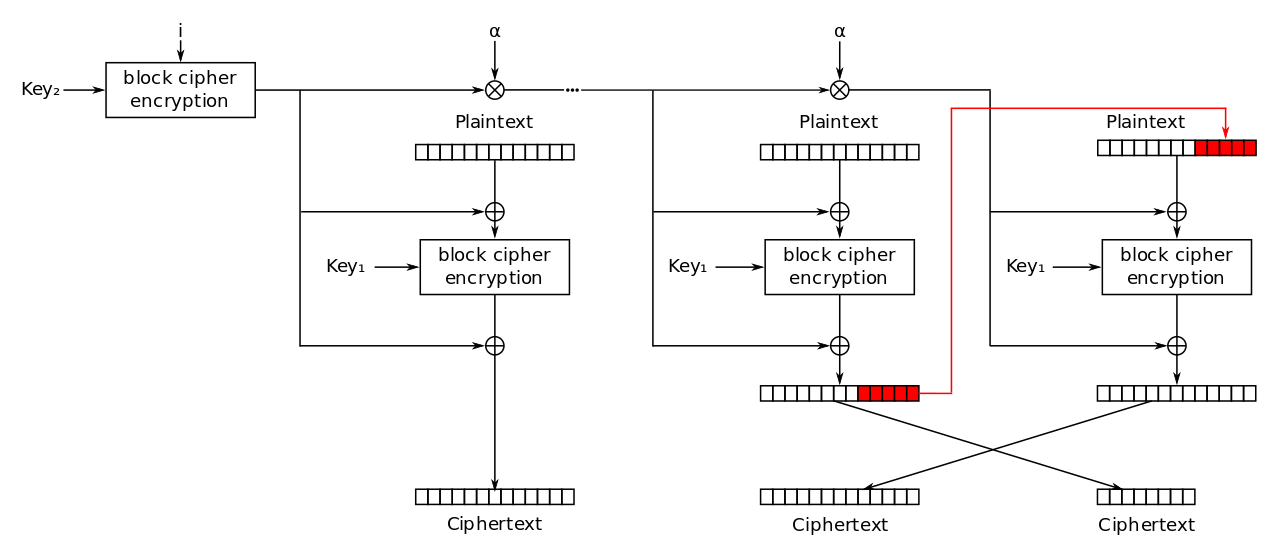
\includegraphics[width=1\textwidth]{XTS_mode_encryption}
    \caption{Schéma XTS algoritmu}
    \label{fig:XTS}
\end{figure}
